\chapter{Introduction}
\label{chapter:introduction}

Events are unorchestrated and asynchronous messages
that carry information in software systems.
They can communicate the states of devices,
signal updates for ongoing or completed processes,
and exchange data with external systems.
They are a fundamental component in
workflow management systems,
cyber-physical operations,
Internet-of-Things devices,
decision support systems,
etc.,
which are ubiquitous in modern society
and are still growing in scale and importance.
Event-based systems produce time-ordered sequences of events,
i.e., event streams,
which demand processing to produce useful information
about the underlying systems for human operators.
Thus,
efficient and effective techniques for processing event streams
are an open problem for research
and a focus of research communities
(e.g., \cite{zhou2022proceedings}).

Workflow management systems
are a class of event-based systems
that automate business processes,
such as order fulfillment and customer service,
by organizing the activities of multiple participants
(e.g., people and software services)
into a coherent workflow.
By enacting workflows,
workflow management systems produce event streams
that serve as a record of the system's execution.
One use of these streams is
to identify exceptional situations,
such as
violations of organizational policies,
regulations, service-level agreements,
or other constraints.
These constraints on workflows
are collectively referred to as {\em (business) rules}.
For example,
a rule may specify that:
{\em Every purchase order must be approved by a manager
before the order is fulfilled},
or
{\em Every customer service request must be resolved within 24 hours}.
Failure to comply with these rules
can result in financial loss,
legal liability,
or in the worst case,
physical harm.

In the last two decades,
static verification (e.g., model checking) has been applied to enforce rule compliance
in a variety of domains \cite{DamaggioDHV:BPM11:verif,CalvanesePODS13}.
In this approach, 
business processes or 
enabling software
are mapped to a formal model,
e.g., a Petri net \cite{du2014timed}
or finite state machines
\cite{BultanSF:IEEEIC,krotsiani2017cloud},
then
all possible behaviors of the model
are checked against rules in a formal specification language,
e.g., linear temporal logic \cite{pnueli1977temporal}.
Unfortunately,
static verification is more difficult to apply
when participants
are allowed flexible behavior,
e.g., a provider or client can initiate processes at arbitrary times.
Including more flexibility
leads to a massive number of possible enactments,
making model checking intractable or undecidable
for expressive classes of rules.
The infeasibility of
preventing rule violations with static verification 
does not indicate a design flaw,
rather it follows from the desired flexibility
of target applications.

An alternative approach to static verification
is {\em runtime monitoring},
where a monitoring mechanism,
often a finite state machine or an online algorithm,
observes the service's execution trace
and detects constraint violations incrementally.
The construction and implementation of monitoring mechanisms from formal specifications
is now a central topic in the field of runtime verification
\cite{barringer2010runtime,bartocci2018introduction,bartocci2019international}.
In one approach,
a monitor is embedded
in application software
\cite{baresi2005towards,fernando2017monitoring},
though this method has disadvantages:
changes to rules require re-engineering
and
the overhead of checking rules
may increase the application's
time and space usage.
% Also, programmatic guards not provide
% an efficient representation of how the enactment
% can be advanced to satisfy the rule.
An alternative approach is
to separate the runtime monitor
from its target application.
This separation
abstracts system-level details
out of the rule specification and
the monitor,
meaning rule changes can be implemented quickly.
Also,
the monitor can be optimized
for the specific task of checking rules,
e.g., using specialized resources
or parallelization,
without affecting the application.

Merely identifying exceptional situations
may not be sufficient to ensure good system behavior;
it is also valuable to identify them {\em at the earliest possible time}.
This allows the system maximum time to take corrective action,
such as removing resources from the offending process.
In extreme cases for safety-critical systems,
late identification could lead to danger for people or property.
To identify the earliest possible violation of an LTL formula,
reference \cite{kupferman2001model} shows that
each violating trace has a minimal prefix
that indicates the violation is inevitable;
early violation detection can be done by recognizing these prefixes at runtime
using finite state machine monitors \cite{giannakopoulou2001automata,bauer2011runtime}.
% or other reasoning techniques \cite{bersani2010smt},
% as well as
% for other languages such as
% Declare \cite{maggi2011runtime, montali2014monitoring}
% and
Some of these techniques
have been extended to handle data in events,
e.g., for constraints in 
first-order linear temporal logic \cite{riccardo2014monitoringfsa, bauer2013propositional}.
However,
these techniques do not address 
quantitative time constraints,
or combinations of 
quantitative time constraints
with constraints on event data,
both of which are common in business rules \cite{ly2015compliance}.

\medskip

In this dissertation,
we focus on early violation detection
for a variety of classes of rules and streams.
We start by developing a framework
for event streams that carry data and timestamps
from completed activities in workflow enactments.
We then define a language
for specifying business rules,
with key features
for specifying quantitative time constraints and conditions on event data (Chapter\:\ref{chapter:preliminaries}),
features (or their combination) that are often missing in existing research
on runtime monitoring and compliance for business rules.
Then,
we describe what it means for an event stream
to satisfy or to violate a set of rules.
Finally,
we illustrate what it means
to detect violations at the earliest possible time:
for a given set of rule and event stream,
a violation is detected at the earliest possible time $t$
if and only if
at all times before $t$,
the stream can be extended by future events to satisfy the set
and all times at and after $t$,
the stream cannot be extended by future events to satisfy the set.
To detect violations at the earliest possible time
is the {\em early violation detection} problem.

Given this framework and problem,
a fundamental question to address is
whether or not it is possible to automate early violation detection.
We show that this is impossible
by showing the related problem of finite satisfiability
is computationally undecidable
(Chapter\:\ref{chapter:finite-satisfiability}).
To prove this,
we use a modified rule language called Datalog$^{+}$
and
reduce the empty-tape Turing machine halting problem
(known to be undecidable)
to determining finite satisfiability for a set of Datalog$^{+}$ rules
constructed from a Turing machine.
Then, we show finite satisfiability
for a set of Datalog$^{+}$ rules
can be reduced to finite satisfiability for a set of rules in our language.
This result indicates that
early violation detection,
though desirable,
is fundamentally intractable,
and thus
the problem requires simplfying assumptions to be solved algorithmically.

To establish feasible cases of early violation detection,
we study subproblems where the sets of rules or event streams
have certain restrictions,
including
when the rules constrain exclusively event timestamps
(and not event data),
when only a single rule is considered,
whether or not the set of rules is acyclic,
i.e., whether or not the dependencies between rules in the target set
form a graph with a cycle,
and
how many events per second are in the stream.
For each of these subproblems,
we develop or improve techniques for early violation detection.

Given our focus on quantitative time constraints,
a natural subclass of rules we consider
are those that only constrain event timestamps
and not event data, i.e., dataless rules;
we describe how early violation detection is possible
through translation from dataless rules to LTL formulas to finite state machines
and provide two translations that improve on existing techniques (Chapter\:\ref{chapter:ltl-translation}).
For the first translation,
we use a graph representation to characterize ``acyclic'' and ``singly-linked'' rules;
the tree structure of acyclic, singly-linked, dataless rules,
allows us to translate the time constraints (if any) on each pair of events in the rule separately,
then combine these into a single translation.
Building on this translation,
we devise a second translation for arbitrary, singly-linked, dataless rules
by leveraging a decomposition of quantitative time constraints into all their possible gaps and orderings,
which reduces the problem to the acyclic case.
The size of the output of these two translations is an LTL formula
whose size is at most single- or double-exponential, respectively, in the size of the input rule,
both improving on the hyper-exponential size of the best known translation.

Using constraints on event data,
e.g., requiring that the same user who makes a request also receives approval,
allows for more expressive rules,
but also makes early violation detection more difficult
because the values of data variables are not known in advance,
and thus
finite state machines alone cannot be used to detect violations;
to address this, we also study rules with data variables,
developing algorithms
based on assignments to these variable
(Chapter\:\ref{chapter:early-violation-detection}).
We define data structures to track potential violations
and present algorithms to update these data incrementally
as new events arrive from the stream.
Notably, we use a chase process,
a well-known technique in database systems,
to reason about dependencies between rules and potential violations,
and
a satisfiability test on linear inequalities
to compute ``deadlines'',
the earliest time at which a violation is inevitable,
that mark permanent violations.
To ensure the chase terminates,
we restrict these algorithms to acyclic sets of rules,
i.e., sets of rules whose dependencies form a directed acyclic graph,
a common restriction when applying the chase process.
To evaluate the effectiveness of these algorithms,
we implemented them in a software runtime monitor
and tested them on a variety of rule sets and event streams
to measure their feasibility, benefits, and limitations.
The evaluation shows that early violation detection can be beneficial
by greatly reducing the number of events that must be processed
to identify violating streams,
and show that our techniques are feasible for medium-scale systems,
e.g., thousands of events per second.

Fortunately,
our techniques for acyclic sets of rules with data variables
can be extended to include aggregation functions,
a common features of business rules that aggregate properties of groups of events,
without affecting the decidability of early violation detection.
In Chapter\:\ref{chapter:aggregation},
we develop a framework for classifying and specifying time windows
on streams and for defining aggregation functions over these windows
in our rule language.
We show that these features,
along with the restriction that the target stream has at most one event per timestamp,
still allow early violation detection for acyclic sets of rules.
To integrate aggregation into our existing algorithms,
we provide two approaches.
First, we present an encoding of aggregation rules as Datalog$_\mathbb{Z}$ programs,
providing a means of evaluating rules with aggregation within a Datalog framework.
Alternatively, we develop techniques to rewrite aggregation expressions over time windows
as Presburger arithmetic formulas,
for which decision procedures exist.
This rewriting allows us to apply a similar chase process and satisfiability testing
to acyclic sets of rules with aggregation functions,
enabling early violation detection.

We organize the dissertation according to the various subclasses of rules considered.
First,
in Chapter\:\ref{chapter:preliminaries},
we present definitions of core concepts.
Then,
the chapters are organized by the the subclasses of rules or sets of rules
they consider,
as shown in Fig.\:\ref{fig:organization}.
Chapter\:\ref{chapter:ltl-translation} studies early violation detection for dataless rules,
Chapter\:\ref{chapter:early-violation-detection}
studies rules with data variables,
Chapter\:\ref{chapter:aggregation} adds aggregation functions over time windows,
and
Chapter\:\ref{chapter:finite-satisfiability}
considers unrestricted sets of rules.

\begin{figure}
    \centering

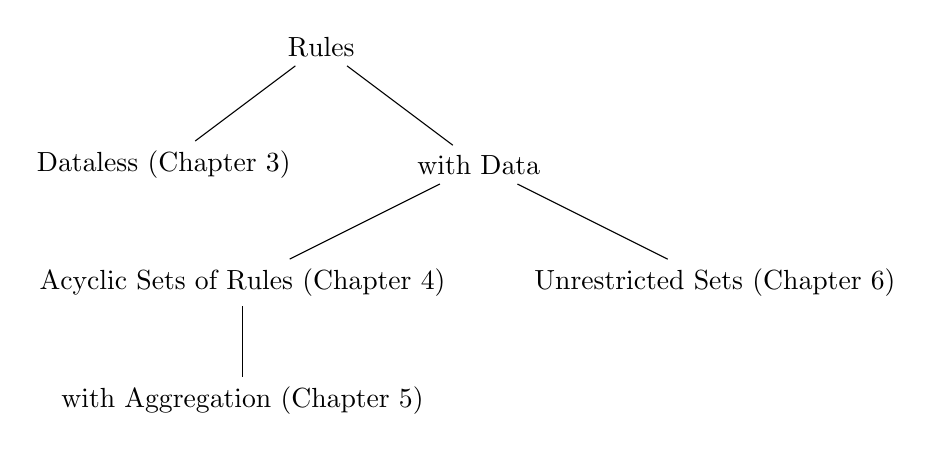
\begin{tikzpicture}[level distance=1.5cm,
    level 1/.style={sibling distance=4cm},
    level 2/.style={sibling distance=6cm}]
    
    \node {Rules}
    child {node {Dataless (Chapter 3)}}
    child {node {with Data}
    child {node {Acyclic Sets of Rules (Chapter 4)}
    child {node {with Aggregation (Chapter 5)}}
    }
    child {node {Unrestricted Sets (Chapter 6)}}
    };
\end{tikzpicture}

\caption{Dissertation organization.}
\label{fig:organization}
\end{figure}

% \begin{section}{Permissions and Attributions}
% \begin{enumerate}
% \item The content of chapter \ref{chapter:translation} has previously appeared in the Elsevier Journal of Information Systems \cite{mackey2023mapping}.
% % It is reproduced here with the permission of (Institution): \url{http://}.
% \end{enumerate}
% \end{section} % Permissions and Attributions
